\documentclass[a0,landscape]{a0poster}
\usepackage{times}
\usepackage{graphicx}
\usepackage{multicol}
\usepackage{geometry}
\usepackage{qrcode}
\usepackage{amssymb}
\usepackage[most]{tcolorbox}
\usepackage{alltt}

% --- Page Geometry (Set to 48x36 inches with a 1-inch margin) ---
\geometry{papersize={48in,36in}, margin=1in}

% --- Custom Box Style ---
\newtcolorbox{posterbox}[1]{
    colback      = blue!5!white,
    colframe     = blue!75!black,
    fonttitle    = \bfseries\huge,
    title        = {#1},
    breakable,
    boxsep       = 8mm,
    arc          = 5mm,
}

\begin{document}

% === TITLE BLOCK ===
\begin{center}
    \veryHuge \textbf{RMSTSS: A New Tool for Planning Better, Faster Medical Studies} \\
    \vspace{0.25cm}
    \rule{\linewidth}{1.5pt}
    \vspace{0.25cm}
    \Huge \textbf{Arnab Aich} \\
    \huge \textit{University of Tennessee Health Science Center}
\end{center}

\vspace{0.5cm}

% === 3-COLUMN LAYOUT ===
\begin{multicols}{3}

% --- COLUMN 1 ---
\begin{posterbox}{What is RMST?}
    \huge
    RMST stands for **Restricted Mean Survival Time**. It measures the average "event-free" time for patients up to a specific follow-up time.

    \subsection*{\Huge Why is it a good measure?}
    \begin{itemize} \itemsep=0.75em
        \item[\Huge\checkmark] \huge It is easy for doctors and patients to understand.
        \item[\Huge\checkmark] \huge It provides a clear, direct measure of treatment benefit.
        \item[\Huge\checkmark] \huge It avoids relying on complex statistical assumptions.
    \end{itemize}
    
    \begin{center}
        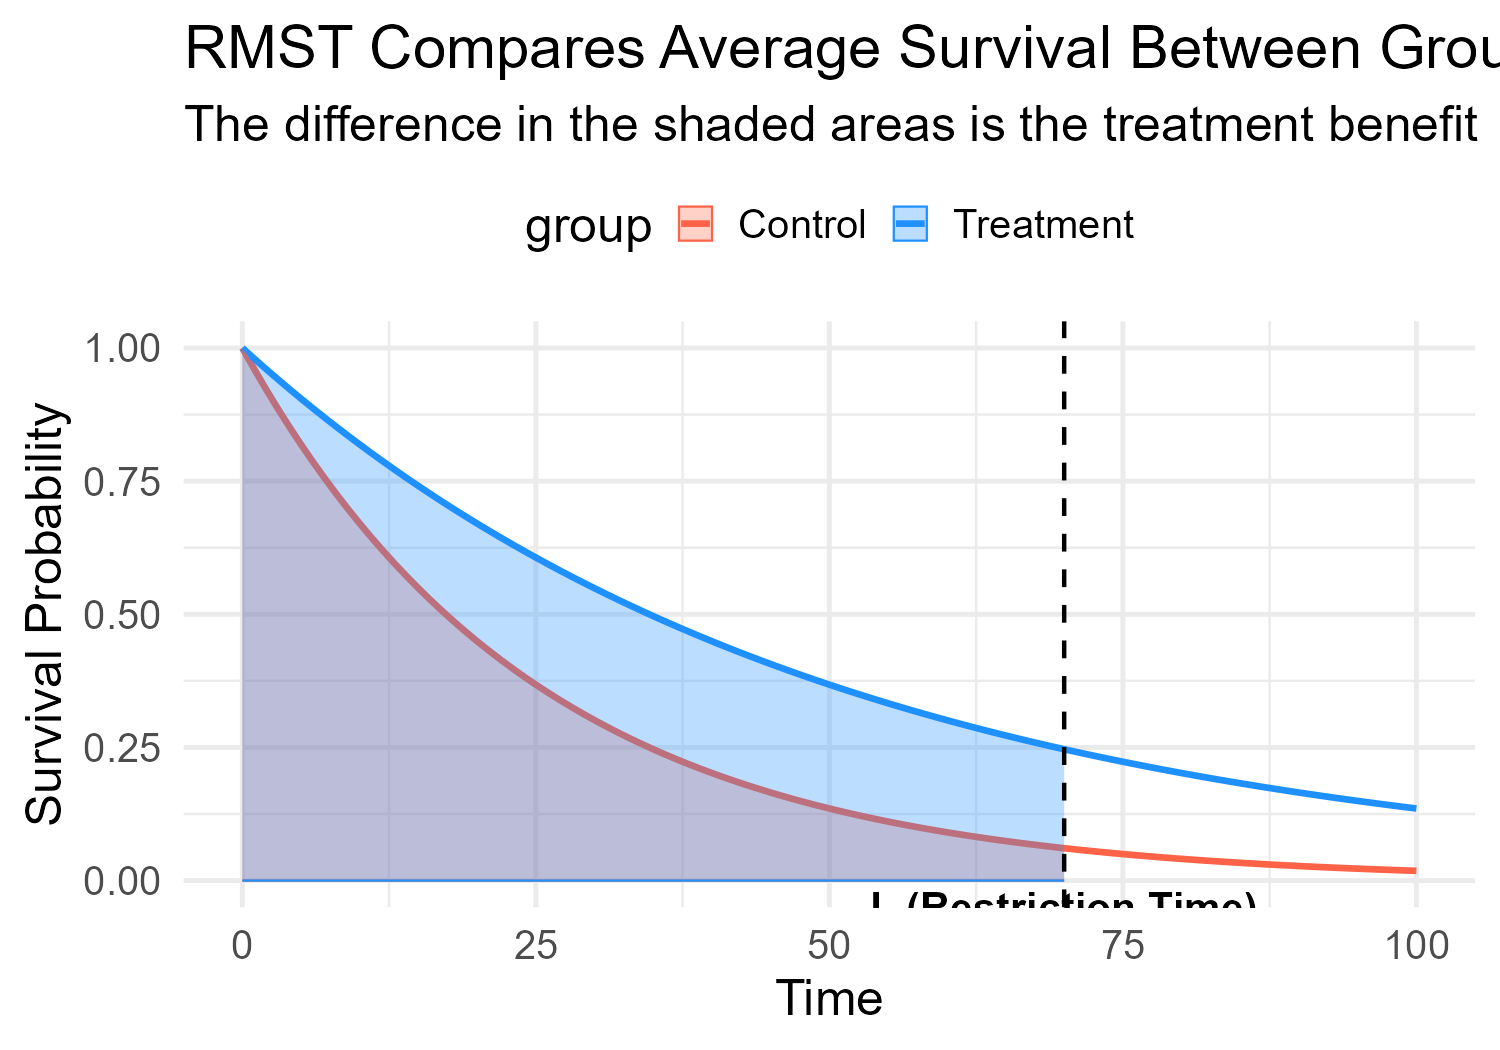
\includegraphics[width=0.9\linewidth]{rmst_causal_plot.png}
    \end{center}
\end{posterbox}

\begin{posterbox}{Our Solution: The RMSTSS Tool}
    \huge
    Planning studies with RMST has been difficult. We made it easy.
    `RMSTSS` is a free tool that helps researchers properly plan modern medical studies. It is available as both an R package and an easy-to-use web application.
    
    \subsection*{\Huge How to Access Our Tool}
    \subsubsection*{\huge For R Users}
    \Large
    Install our R package to use these calculations in your code.
    \begin{alltt}
remotes::install_github(
  "UTHSC-Zhang/RMSTSS-Package"
)
    \end{alltt}

    \subsubsection*{\huge For Everyone Else}
    \Large
    Use our web application. No installation or coding needed!
    \begin{center}
        \qrcode[height=4cm]{https://arnab96.shinyapps.io/uthsc-app/}
        
        \textbf{\huge Scan to use the web app}
    \end{center}
\end{posterbox}

\columnbreak

% --- COLUMN 2 ---
\begin{posterbox}{Features \& Capabilities}

    \subsection*{\Huge A Full Suite of Modern Models}
    \huge
    Our tool handles many real-world research scenarios:
    \begin{itemize} \itemsep=0.75em
        \item \textbf{Linear Model}: For standard clinical trials.
        \item \textbf{Stratified Models}: For studies run at many different hospitals.
        \item \textbf{GAM Model}: For studies where factors like patient age have complex effects.
        \item \textbf{Dependent Censoring}: For studies with competing outcomes, like transplants.
    \end{itemize}

    \subsection*{\Huge Choose Your Goal}
    \huge
    \begin{itemize} \itemsep=0.75em
        \item \textbf{Power Calculation}: Find the chance of success for a given study size.
        \item \textbf{Sample Size Search}: Find how many patients you need to succeed.
    \end{itemize}

    \subsection*{\Huge Choose Your Method}
    \huge
    \begin{itemize} \itemsep=0.75em
        \item \textbf{Quick Check (Analytical)}: A fast answer for exploring ideas.
        \item \textbf{Deep Dive (Bootstrap)}: A powerful simulation for a more accurate result. Our tool can run these simulations in parallel to be faster!
    \end{itemize}

\end{posterbox}

\columnbreak

% --- COLUMN 3 ---
\begin{posterbox}{How the App Works}
    \huge
    The web application guides you through the process in a few simple steps.
    \begin{center}
        \Huge
        \textbf{1. Upload Data} \\[1cm]
        $\boldsymbol{\downarrow}$ \\[1cm]
        \textbf{2. Choose Your Model \& Goal} \\[1cm]
        $\boldsymbol{\downarrow}$ \\[1cm]
        \textbf{3. Get Instant Results!}
    \end{center}
    \huge
    The app provides interactive plots, summary tables, and downloadable PDF reports.
\end{posterbox}

\begin{posterbox}{Learn More \& Get in Touch}
    \subsection*{\Huge Future Scope}
    \huge
    We are always improving the `RMSTSS` tool, with plans to add more bootstrap methods and advanced diagnostic tools.

    \subsection*{\Huge Project Page}
    \huge
    Visit our GitHub page for the source code and documentation.
    \begin{center}
        \qrcode[height=4cm]{https://github.com/UTHSC-Zhang/RMSTSS-Package}
        
        \textbf{\huge Scan for the GitHub Project}
    \end{center}

    \subsection*{\huge Key References}
    \Large
    Royston \& Parmar (2013), Tian et al. (2014), Uno et al. (2014), Wang et al. (2018, 2019), Zhang \& Schaubel (2024).
\end{posterbox}

\end{multicols}
\end{document}